\documentclass[10pt,a4paper]{article}
\usepackage[latin1]{inputenc}
%\usepackage{url}
%\usepackage{booktabs}
\usepackage{amsmath}
\usepackage{amsfonts}
\usepackage{amssymb}
\usepackage{subfigure}
\usepackage{graphicx}
\graphicspath{{imgs/}}

\usepackage{xspace}
\newcommand*{\eg}{e.g.\@\xspace}
\newcommand*{\ie}{i.e.\@\xspace}
\newcommand*{\ea}{et al.\@\xspace}
\renewcommand{\arraystretch}{1.5}

\newcommand{\prob}{Pr}
\newcommand{\rgbdimage}{\mathbf{I}}
\newcommand{\imregion}{\mathcal{R}}
\newcommand{\occ}{o}
\newcommand{\basisshape}{B}
\newcommand{\pcloud}{\mathcal{P}}
\newcommand{\point}{\mathbf{p}}
\newcommand{\normal}{\mathbf{n}}

\title{Predicting Scene Voxel Occupancy From a Single RGBD Image}

\author{Michael Firman}

\begin{document}
\maketitle


\abstract{
	We present a method to predict, given a single RGBD image, the voxel occupancy of each voxel in the scene. We make these predictions for this ill-posed problem using a database of CAD shapes, which we consider to be generic enough to be used to describe shape.

}


\section{Introduction}

Single image - get a good overview of the scene and what is going on. However, only see a very small subset of the surfaces in the scene. (Blender image?), and can only directly infer a very small number of occupied voxels. 
Very useful to know if voxels are occupied, for various reasons.

Reasons for occlusions. Self occlusions. Hidden underneath. Etc.

Given a single RGBD image, the aim of this system is to predict whether each voxel in the scene is occupied or not - in effect, we want to predict the output of KinectFusion, but having been given only a single view of the scene instead of multiple views.

We [plan to] achieve this by matching regions from the input image to renders of objects in a training database.
The voxel occupancy of these objects can then be combined together to give a prediction for each of the voxels in the scene. 
Because we care about voxel occupancy, and not semantic understanding, we are free to use training objects which differ in scale and semantic labelling from the objects being modelled in the scene. 
This is key to our approach --- we are not reasoning about semantics of objects, but instead about object shape.
In effect we are hypothesising that any two objects that have a similar shape from one angle are likely to share similarities in shape in the unobserved regions of the scene.

Of course the problem is ill-posed, compared to well-posed problems such as reconstruction. 
We therefore can only hope to make a reasonable guess of the occupancy, and rely on the predictability and repeatability of the world.


This has applications in:

\begin{description}

\item[Robotics] --- Helping a robot to plan a path around objects given only a single view of a scene, e.g. from a doorway. Also to help a robot plan grasping position on objects it can only see partial views of.

\item[Scene relighting] --- Enabling realistic-looking shadows to be cast from a light moved to a new position in the image.

\item[Object repositioning] --- Interactive repositioning of objects in the scene. Knowing the voxel occupancy allows a constraint to be placed on where objects can be moved to. (\eg Zheng \ea, Interactive images)

\item[Re-rendering scene from a new viewpoint]
\end{description}

In addition, our output can act as a prior for algorithms such as registration.


\subsubsection{What is our hypothesis?}

What is our overall hypotheses --- that the shape we can see from one angle is enough information to make a sensible prediction about the parts of the scene which are occluded?

We aren't making assumptions about class, unlike \eg shotton (people) or room modelling.

\subsubsection{Motivation for using a voxelised world}

Voxels are expensive compared to point clouds and meshes. 
However they are a very natural representation of our world, and have been shown to work well for reconstruction \eg KinFu, other voxel carving paper. 

\begin{quote}
Voxel occupancy is one approach for reconstructing the 3-dimensional shape of an object from multiple views. In voxel occupancy, the task is to produce a binary labeling of a set of voxels, that determines which voxels are filled and which are empty.

\cite{snow-cvpr-2000}
\end{quote}

In addition, our world remains at the same resolution, while computers are becoming larger and more powerful. 
People have make work-arounds for efficiently using voxels in very large ares, \eg Kintinuous.



\begin{figure}
	\centering 
	\subfigure[Example input image]{%
		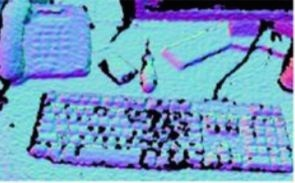
\includegraphics[width=0.4\columnwidth]{kinfu1.jpg}}
		\hfill
	\subfigure[Ground truth output]{%
		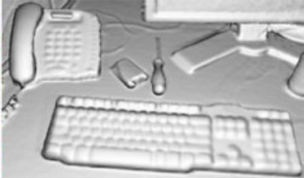
\includegraphics[width=0.4\columnwidth]{kinfu2.jpg}} \\
	\caption{Given a single RGBD image (\eg (a)), the aim is to predict the full, occupied volume of the scene (e.g. (b)).}
\end{figure}

\subsection{Problem statement}

Setting out the problem mathematically, introducing some notaion etc.

What exactly do we mean by voxel occupancy? 

%%%%%%%%%%%%%%%%%%%%%%%%%%%%%%%%%%%%%%%%%%%%%%%%%%%%%%%%%%%%%%%%%%%%%%%%%%%%%%%%
\section{Related work}
%%%%%%%%%%%%%%%%%%%%%%%%%%%%%%%%%%%%%%%%%%%%%%%%%%%%%%%%%%%%%%%%%%%%%%%%%%%%%%%%

\cite{shen-tog-2012} use an assembly of parts from a CAD database to complete the unseen parts of a model given an RGBD image. 
While they demonstrate good results they assume they have semantic-specific models of the objects in the dataset.
Kim \ea \cite{kim-iccv-2013} use a CRF model over a voxel representation of a scene to simultaneously predict occupancy, visibility and semantical labelling of voxels from an RGBD image. 
For training, the use manually labelled top-down views of the scene. 
Their prediction of occupancy, however, is really just a gaussian model. 
Final labellings found from graph cuts over the CRF. 
They make the observation that the observed values from a Kinect sensor can be very bad, and may need cleaning up.

\paragraph{Mesh completion}
In the graphics community, there is a lot of work looking at the completion of missing and occluded parts of 3D meshes. 
For example, \cite{podolak-esgp-2005} fill holes in a mesh by enforcing watertightness across an octree structure, while \cite{schnabel-eurographics-2009} complete meshes by using primitives extracted from the areas of the scan without missing detail. 
A good overview of such mesh completion algorithms are given in \cite{ju-cst-2009}.

\paragraph{Superresotion}
Similar to mesh completion is super-resolution. \eg \cite{macaodha-eccv-2012}. 
Like our problem, super-resolution is ill-posed and relies on the repeatability and predictability of the world in order to find suitable matches.

\paragraph{Symmetry}
Law and Aliaga \cite{law-cviu-2010} use symmetry to complete partial views. 
They are limited to only completing partial views; they rely on all objects being symmetrical; and they need user input.
Similarly, \cite{thrun-iccv-2005} uses symmetry to complete models from a single depth view. 
Uses a great probablistic interpretation of the model view from a depth scene, but again relies on the objects being symmetric.

\paragraph{Indoor room semantic prediction}
These works in general try to understand the semantic layout of a scene, \ie given an image infer what objects are in the scene and what their poses are.
\cite{nan-acm-2012, minkim-siggraphasia-2012}
This could be seen as finding one-to-many correspondences between models in a database and points in the scene.

\paragraph{Indoor room occupied space prediction}
\cite{hedau-cvpr-2012} seek to recover the free space in 2D images. They label ~500 images with box annotations, and aim to recover the bounding box layout of the scene in order to recover the free space.

In the vision community, most of the work is based around estimating the spatial layout of rooms from images.
For example \cite{bao-wacv-2014} use multiple images, before SfM and segmentation of the images. 
They then generate hypotheses of the layout. 
The hypotheses are chosen by evaluating their geometric cost, which is manually defined. 
They cite a lot of papers which do scene reasoning from a single image, but they argue that the problem is ill-posed (which it is). 

Using a single image, many people fit bounding boxes and try to estimate the layout using high lever info about gravity, typical scene arrangements etc. 
For example \cite{choi-cvpr-2013}.

\cite{lee-nips-2010} are another paper using a single image to estimate the layout of a room. 
Similarly, \cite{zhang-iccv-2013} infer the clutter and layout and support and segmentation and labelling from an RGBD image (using the NYU dataset).

\cite{hedau-cvpr-2012} seek to recover the free space in 2D images. 
They label ~500 images with box annotations, and aim to recover the bounding box layout of the scene in order to recover the free space. 
A big work in this area is that by \cite{gupta-cvpr-2011}, who estimate voxel occupation before fitting boxes.


\paragraph{General motivation}
One key motivation is Shape Sharing \cite{kim-eccv-2012}, where silhouettes of objects are used to segment other objects from different classes.
 \cite{nan-acm-2012}.

Big issue with ground truth. Most papers don't have proper ground truth and therefore can only really do qualitative results, \eg \cite{all the papers...}.


\begin{itemize}
\item Should also cite Oisin.
\item Also the guy who spoke at MSR Cambridge.
\end{itemize}


%%%%%%%%%%%%%%%%%%%%%%%%%%%%%%%%%%%%%%%%%%%%%%%%%%%%%%%%%%%%%%%%%%%%%%%%%%%%%%%%
\section{Methodology}
%%%%%%%%%%%%%%%%%%%%%%%%%%%%%%%%%%%%%%%%%%%%%%%%%%%%%%%%%%%%%%%%%%%%%%%%%%%%%%%%

Overview of the method --- cite \ref{fig:pipeline}.

General motivation for method. Do not want to rely on having exact matches in training set. 
Instead, want to find a collection of good matches in the training set which, when combined, will give a sensible prediction of the voxel occupancy.
We take a RANSAC-style approach to finding basis shapes: first we \emph{propose} a set of candidate shapes which roughly match the scene, before we next \emph{re-weight} these candidates according to how well they match the scene geometry. 

\begin{figure}
	\centering 
	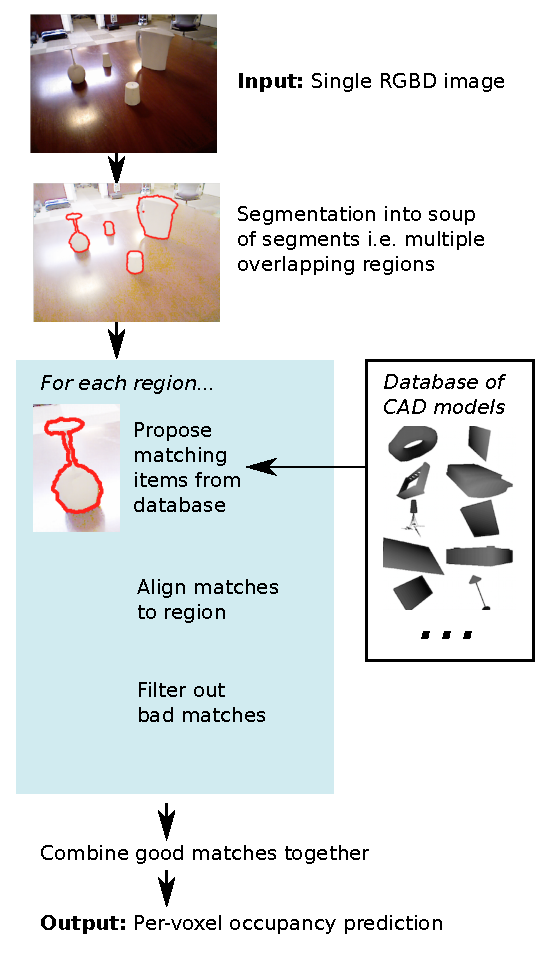
\includegraphics[width=0.6\columnwidth]{pipeline}
	\caption{The pipeline used --- work in progress!}
	\label{fig:pipeline}
\end{figure}

\subsection{Prediction voxel occupancy}
The ultimate aim is to predict, for each voxel in the scene, the probably of the event $\occ$, \ie the probability that it is occupied or not. We therefore want $\prob(\occ_k | \rgbdimage)$.
$$
\prob(\occ_k | \rgbdimage) = \sum_{i,j} \prob(\occ_k|\basisshape_i)\prob(\basisshape_i|\imregion_j)\prob(\imregion_j|\rgbdimage)
$$

\begin{itemize}
\item $\prob(\occ_k|\basisshape_i)$ ---
This is $1$ if the voxel is inside the transformed basis shape mesh, and $0$ otherwise.
\item $\prob(\basisshape_i|\imregion_j)$ ---
This is the probability that basis shape $\basisshape_i$ is a correct match for region $\imregion_j$. We approximate this based on how well the region $\imregion_j$ matches the visible part of the $\basisshape_i$.
\item $\prob(\imregion_j|\rgbdimage)$ ---
This is the probability that the region of the image $\imregion_j$ is a correct segmentation of image $\rgbdimage$.
\end{itemize}


%%%%%%%%%%%%%%%%%%%%%%%%%%%%%%%%%%%%%%%%%%%%%%%%%%%%%%%%%%%%%%%%%%%%%%%%%%%%%%%%
\subsection{A soup of segments}

Our motivation for using a soup of segments together with class matching across class boundaries is like this. 
Imagine we had a chair in our test set. If in our training set we had a similar chair then we would like to use this, as it would hopefully be a good match. 
However, if we didn't have a chair in our training set then it is very unlikely that we would be able to find a suitable match. 
In this case, we would like to break up the chair into segments, each of which could have a similarly shaped object matched to it.

%%%%%%%%%%%%%%%%%%%%%%%%%%%%%%%%%%%%%%%%%%%%%%%%%%%%%%%%%%%%%%%%%%%%%%%%%%%%%%%%
\subsection{Finding matches for each region}

Find the $n$ nearest neighbours in $\chi^2$ distance space.

%%%%%%%%%%%%%%%%%%%%%%%%%%%%%%%%%%%%%%%%%%%%%%%%%%%%%%%%%%%%%%%%%%%%%%%%%%%%%%%%
\subsubsection{Features}

Simple pairwise features very popular in RGBD image understanding, e.g. Drost, Shotton, Microsoft 7-scenes, FPFH, KinFu... 
We use variants on the shape distribution \cite{osada-csma-2001} to form our FV. 
Given a point cloud $\pcloud = \{\point_1, \hdots, \point_N\}$ with associated normals $\{\normal_1, \hdots, \normal_N\}$ we select random pairs of 
$$
\mathbf{f}_{i,j} = \left(|\point_i, \point_j|_2, \angle(\normal_i, \normal_j)\right),
$$
where $\angle(\normal_i,\normal_j)$ denotes the angle in radians between the normal vectors $\normal_i$ and $\normal_j$.
We use the bag-of-words approach to aggregate the features for an entire region, into a feature vector. We use a dictionary with 75 words, formed using k-means.

We don't necessarily have an exact match for each region or object in the database. We therefore allow for there to be 

\paragraph{Scale invarience}
We want to allow for scale invariance. To allow for this we rescale the points in each region and basis shape render by $s$, where $s$ is the 95th percentile of the pairwise distances in the region.

\subsection{Finding matches for each region}


\subsection{Combining matches together}



\subsection{For single object, single segmentation.}

Image is $\rgbdimage$, event of occupancy is $o$. Basis shape is $\basisshape$.
$$
\prob(\occ | \rgbdimage) = \sum_i \prob(\occ | \basisshape) \prob(\basisshape | \rgbdimage)
$$ 
We know that $\prob(\occ|\basisshape)$ is just 1 within the shape, and 0 outside. 
$\prob(\basisshape|\rgbdimage)$ is harder but could be based on some kind of heuristic based on number of inliers and how well the shape matches in etc.

In particular:
$$ 
\sum_i \prob(\basisshape|\rgbdimage) = 1
$$

\subsection{For multiple segmentations.}

Now we have to introduce the concept of segmentations. 
The image $\rgbdimage$ will be segmented into a number of different regions $R$, where these regions may (but need not) overlap and the union of the regions need not cover the whole image.

We can then perform the fitting as before, but this time on a per-region basis. The regions are then marginalised out:
$$
\prob(\occ | \rgbdimage) = \sum_{i,j} \prob(\occ|\basisshape)\prob(\basisshape|\imregion_j)\prob(\imregion_j|\rgbdimage)
$$

Similar to before,
$$
\sum_i \prob(\basisshape|\imregion) = 1
$$

However, there is no obligation for $\sum_j \prob(\imregion_j | \rgbdimage) = 1$, as the regions may be non-overlapping.

The only thing left to compute is the probability of a specific region given the image, i.e. $\prob(\imregion_j|\rgbdimage)$. 

$$
\prob(\imregion_j | \rgbdimage) = \sum_{k} \prob(\imregion_j|S_k)\prob(S_k|\rgbdimage)
$$
$\prob(\imregion_j | S_k)$ is just the probability 


%%%%%%%%%%%%%%%%%%%%%%%%%%%%%%%%%%%%%%%%%%%%%%%%%%%%%%%%%%%%%%%%%%%%%%%%%%%%%%%%
\section{Experiments}
%%%%%%%%%%%%%%%%%%%%%%%%%%%%%%%%%%%%%%%%%%%%%%%%%%%%%%%%%%%%%%%%%%%%%%%%%%%%%%%%

\subsection{Database of CAD models}
Use the database from Fisher \ea \cite{fisher-siggrraphasia-2012}.
1600 CAD models, each depth-rendered from 42 viewing angles using OpenGL.


%\bibliographystyle{plain}
\bibliographystyle{apalike}
\bibliography{bibtex/strings.bib,bibtex/main.bib,bibtex/crossrefs.bib}

\end{document}